\chapter{Temo:  Spongo de Menger}

{ }\hfill\textbf{Nivelo:} Alta

En ^ci tiu ^capitro, ni konstruos solidan fraktalon nomatan
\emph{spongo de Menger}.  Jen la unuaj iteracioj por konstrui tiun
solidon:

\begin{center}
  \begin{minipage}{6cm}
    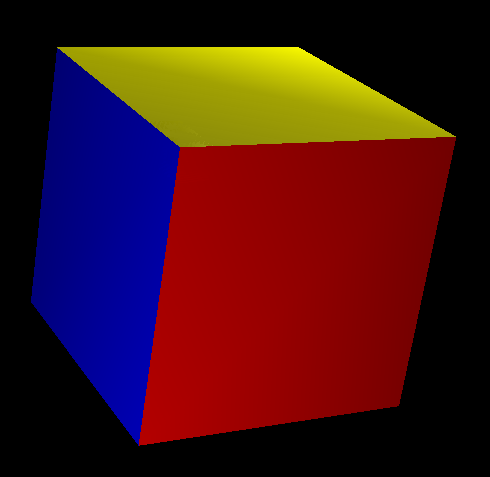
\includegraphics[width=6cm]{bildoj/menger0.png}
    \begin{center}
      \textbf{Stadio 0}
    \end{center}
  \end{minipage}
  \begin{minipage}{6cm}
    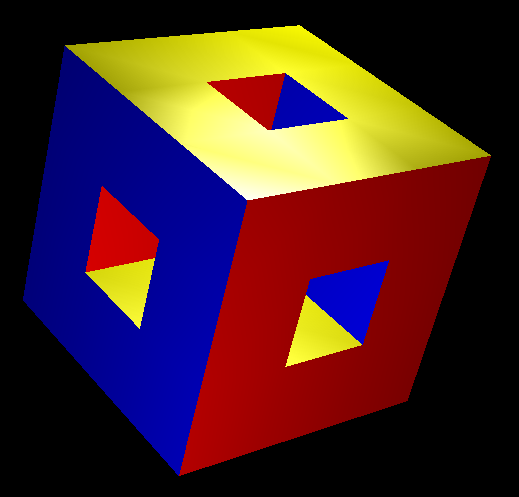
\includegraphics[width=6cm]{bildoj/menger1.png}
    \begin{center}
      \textbf{Stadio 1}
    \end{center}
  \end{minipage}
  \\
  \begin{minipage}{6cm}
    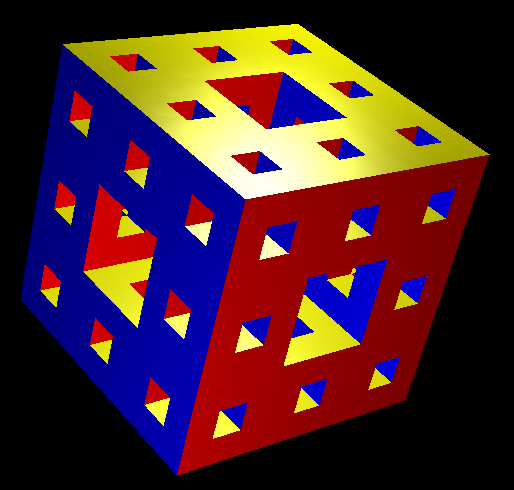
\includegraphics[width=6cm]{bildoj/menger2.png}
    \begin{center}
      \textbf{Stadio 2}
    \end{center}
  \end{minipage}
  \begin{minipage}{6cm}
    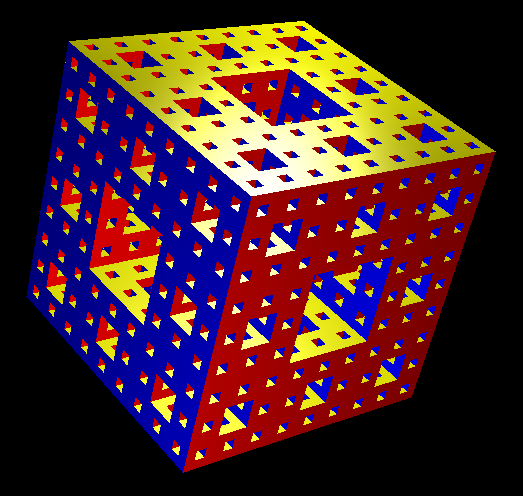
\includegraphics[width=6cm]{bildoj/menger3.png}
    \begin{center}
      \textbf{Stadio 3}
    \end{center}
  \end{minipage}
\end{center}

La ^capitro konsistas el du partoj:
\begin{itemize}
\item Anta^u ^cio, ni montros kiel krei tiun solidon facile per uzo
  de rekursiveco.
\item Poste, oni provos plibonigi la grafikadon por grafiki spongon de
  Menger de ordo~4.
\end{itemize}

\section{Uzante rekursivecon}

Konsideru spongon de Menger de ordo $n$ kies latero mezuras $L$.\\
\begin{center}
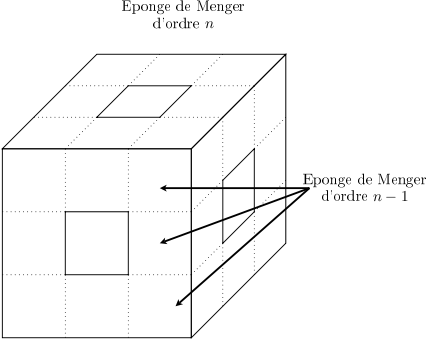
\includegraphics{bildoj/menger-schema01.png}
\end{center}
La skemo montras bone ke tiu spongo konsistas efektive el $20$ spongoj
de Menger de ordo $n-1$ havantaj ^ciuj lateron je ${L}/{3}$.  La
rekursiva strukturo de la spongo evidenti^gas tiel.

\textbf{La programo:}

\begin{verbatim}
# Ĉefa komando: spongo 3
por kubo :l
se :nombrilo = 10000 [tridimensie_vidigu]
# Koloroj de la flankaj facoj
lokp "koloroj [flavan violruĝan verdbluan bluan]
# flankaj facoj
ripetu 4 [skolp ekzek eron kmpt :koloroj kvadrato :l dn 90 an  :l mdn 90 dkn 90]
# Sube
skolp ruĝan malsupren 90 kvadrato :l supren 90
av :l msn 90 skolp verdan kvadrato :l sn 90 man :l
fino

por kvadrato :c
provizu "nombrilo :nombrilo + 1
por_edro
ripetu 4 [an :c dn 90]
fino_edro
fino

# Spongo de Menger
# p: profundeco de rekursiveco
# l: longeco de la granda kubo
por menger :l :p
se :p=0 [kubo :l] 
 [lokp "p :p-1  
  lokp "l :l/3
  # antaŭa faco
  ripetu 3 [menger :l :p an :l] man 3*:l
  dn 90 an :l mdn 90
  menger :l :p an 2*:l menger :l :p man 2*:l
  dn 90 an :l mdn 90
  ripetu 3 [menger :l :p av :l] man 3*:l
  # dekstra flanko
  malsupren 90 an :l supren 90 
  menger :l :p an 2*:l menger :l :p re 2*:l
  malsupren 90 an :l supren 90 
  ripetu 3 [menger :l :p an :l] man 3*:l
  mdn 90 an :l dn 90
  menger :l :p an 2*:l menger :l :p man 2*:l
  mdn 90 an :l dn 90
  ripetu 3 [menger :l :p an :l] man 3*:l
  malsupren 90 man :l supren 90
  menger :l :p an 2*:l menger :l :p man 2*:l
  malsupren 90 man :l supren 90]
fino

por spongo :p
ev tdk provizu "nombrilo 0 perspektive fkolp 0 menger 800 :p 
tajpu [Nombro de kvadratoj: ] s :nombrilo
tridimensie_vidigu
fino
\end{verbatim}

Tiu programo konsistas el kvar proceduroj:
\begin{itemize}
\item \texttt{kvadrato :c}\\
  Tiu proceduro grafikas kvadraton kun lateroj longaj je \texttt{:c}.
  Krome, tiun kvadraton registras la modelilo 3D.  La variablo
  \texttt{nombrilo} responsas pri nombri la nombron de kvadratojn
  desegnitajn.
\item \texttt{kubo :l}\\
  Tiu proceduro grafikas kubon kun lateroj longaj je \texttt{:l}.
  Kompreneble, ^gi uzas la proceduron \texttt{kvadrato}.
\item \texttt{menger :l :p}\\
  Tiu proceduro estas la ^cefa^jo de l' programo; ^gi desegnas motivon
  de Menger de ordo $p$ kaj do la latero mezuras $l$.  Tiun motivon
  oni kreas la^u rekursiva maniero tute nature sekvante la anta^uan
  skemon.
\item \texttt{spongo :p}\\
  Tiu proceduro grafikas spongon de Menger de ordo $p$ kaj kun latero
  $800$ kaj aldonas ^gin al modelilo 3D.
\end{itemize}
\vfill
\pagebreak

\section{Dua pritrakto: solida objekto de $4$-a ordo}

La anta^ua programo havas kiel ^cefan avanta^gon ekspluati la nature
rekursivan strukturon de la fraktala solido.  Rimarku ke tiu sama
metodo povas esti uzata anka^u por generi aliajn fraktalajn solidojn
a^u, pli simple, aliajn fraktalajn kurbojn.  ^Ciuokaze, la tuja
konsekvenco de la rekursiva pritrakto estas mallonga fontokodo kaj
simple komprenebla.  Beda^urinde, rimarku ke spongo je $3$-a ordo
postulas jam $48\,000$ kvadratojn.  Necesas tiam estigi la memoron
dediĉitan al XLogo je $256$ MB en la fenestro pri preferoj por ke la
programo povu ruli^gi tute.

Se oni deziras grafiki Menger-an spongon je $4$-a ordo, balda^u oni
estos barita de for^cerpado de memoro.  En ^ci tiu parto ni vidos
programon bazitan sur tute malsama algoritmo; ^gi ebligos krei spongon
de Menger je ordo $0$, $1$, $2$, $3$ a^u $4$.

\subsection{La tapi^so de Sierpinski}

La spongo de Menger estas efektive ^generaligon en $3$ dimensioj de
ebena figuno nomata \emph{tapi^so de Sierpinski}.  Jen la unuaj
iteracioj de tiu figuro:

\vspace{5mm}
\begin{minipage}{4.1cm}
\begin{center}
 
\includegraphics[width=4.0cm]{bildoj/carpet0.png}\\
\textbf{Stadio 0}
\end{center}
\end{minipage}
\begin{minipage}{4.1cm}
\begin{center}
 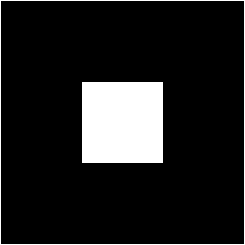
\includegraphics[width=4.0cm]{bildoj/carpet1.png}\\
\textbf{Stadio 1}
\end{center}
\end{minipage}
\begin{minipage}{4.1cm}
\begin{center}
 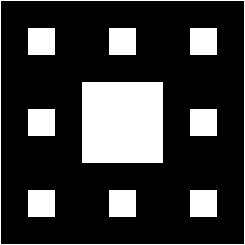
\includegraphics[width=4.0cm]{bildoj/carpet2.png}\\
\textbf{Stadio 2}
\end{center}
\end{minipage}
\begin{minipage}{4.1cm}
\begin{center}
 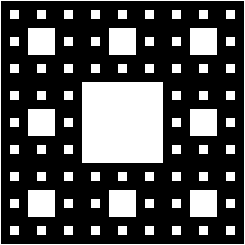
\includegraphics[width=4.0cm]{bildoj/carpet3.png}\\
\textbf{Stadio 3}
\end{center}
\end{minipage}
\vspace{5mm}

La motivo estanta sur ^ciu faco de spongo de Menger je ordo $p$-a
estas tapi^so de Sierpinski je ordo $p$-a.

\subsection{Grafiki tapi^son de Sierpinski je ordo $p$-a}

La celo estas atingi malpligrandigi la nombron de postulitaj kvarlateroj
por desegni tapi^son de Sierpinski.  La jena ekzemplo klarigas la la
procedon uzitan por krei tapi^son de Sierpinski je ordo $3$-a.  ^Ci
tie, la komenca kvadrato konsistas do el $3^3=27$ horizontaloj kaj
$27$ vertikaloj.  Oni skribas je bazo $3$ la numeron de ^ciu
horizontalo kaj ^ciu vertikalo.

\begin{itemize}
\item [\textbullet]\textbf{Unua stadio:} Por ^ciu horizontalo kies
  numero konsistas el neniu $1$, grafiku horizontalon de $27$ ^celoj.
  Pro simetrio, efektivigu la saman operacion vertikale.
\begin{center}
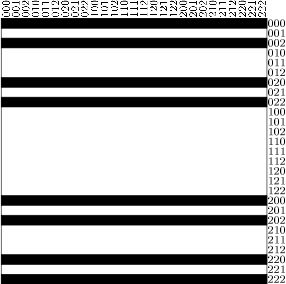
\includegraphics{bildoj/menger-schema02.png}
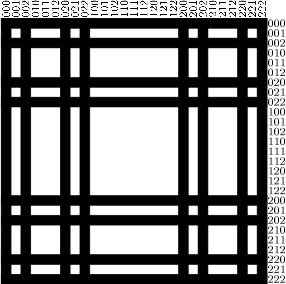
\includegraphics{bildoj/menger-schema03.png}
\end{center}
\vspace{0.2cm}
\item [\textbullet] \textbf{Dua stadio:} Nun interesi^gu pri la
  horizontaloj kies numero konsistas el ununura $1$ en l' unua loko.
  Grafiku sinsekve alterne ortangulojn longaj je $9$ ^celoj.  Faru
  por la vertikaloj simetrie.
\begin{center}
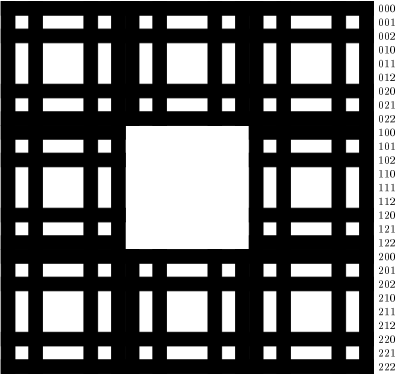
\includegraphics{bildoj/menger-schema04.png}
\end{center} 
\item [\textbullet] \textbf{Tria stadio:} Nun interesi^gu pri la
  horizontaloj kies numero konsistas el nur unu $1$ en la dua loko.
  Grafiku sinsekve alterne ortangulojn la^u la skemo $[3\ 3\ 6\ 3\ 6\
  3\ 3]$ ($3$ ^celoj plenaj, $3$ malplenaj, $6$ plenaj, ktp...).
  Simetrie faru por la vertikaloj.
\begin{center}
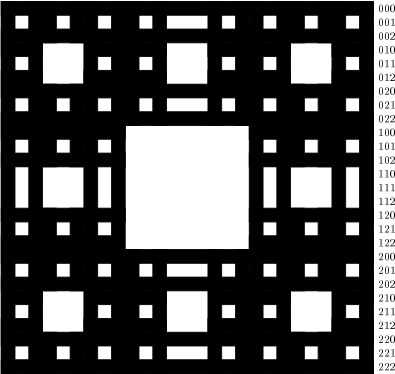
\includegraphics{bildoj/menger-schema05.png}
\end{center}
\item [\textbullet] \textbf{Lasta stadio:} Interesi^gu pri
  horizontaloj kies numero konsistas el du $1$ lokitaj en l' unuaj
  lokoj.  Grafiku sinsekve alterne ortangulojn la^u la skemo $[3\ 3\
  3\ 9\ 3\ 3\ 3]$.  Operaciu same por la vertikaloj.
\begin{center}
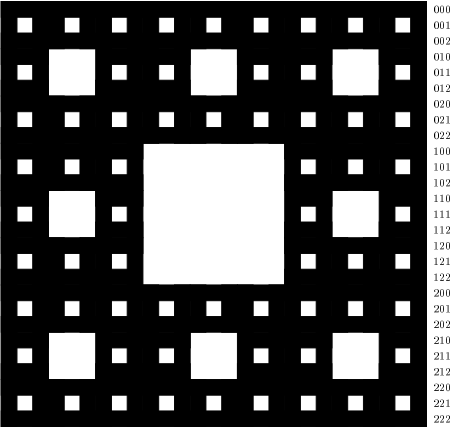
\includegraphics{bildoj/menger-schema06.png}
\end{center}
\end{itemize}
Tiam fini^gas la konstruado de la tapi^so de Sierpinski je ordo $3$-a.
Por krei tiun tapi^son necesis uzi entute: $16+16+32+16=80$
ortangulojn.

\subsection{Malsamaj skemoj de vertikaloj eblaj}

Por resumi la anta^uan konstruadon, jen la malsamaj tipoj de skemaj de
vertikaloj la^u ilia numero.  (La simbolo * indikas la ciferon $0$ a^u
la ciferon $2$.
\begin{center}
  \begin{tabular}{|c|c|}
    \hline
    Numero de la tipo & Skemo aplikenda \\
    \hline
    *** & 27 \\ 
    \hline
    1** &  9 9 9 \\
    \hline
    *1* & 3 3 6 3 6 3 3\\
    \hline
    11* & 3 3 3 9 3 3 3\\
    \hline
  \end{tabular}
\end{center}

Sur la sama principo, por krei tapi^son je ordo $4$-a, oni uzu
kvadraton kun $3^4=81$ ^celoj.  La numeroj de horizontaloj kaj
vertikaloj havos do $4$ ciferojn en ilia prezentado je bazo $3$.  Por
^ciu tipo de numero, jen la skemo aplikenda (la simbolo * indikas la
ciferon $0$ a^u la ciferon $2$):

\begin{center}
 \begin{tabular}{|c|c|}
 \hline
Numero de tipo & Skemo aplikenda \\
\hline
 **** & 81 \\ 
\hline
1*** &  27 27 27 \\
\hline
*1** & 9 9 18 9 18 9 9 \\
\hline
**1* & 3 3 6 3 6 3 6 3 6 3 6 3 6 3 6 3 6 3 3 \\
\hline
*11* &  3 3 3 9 3 3 6 3 3 9 3 3 6 3 3 9 3 3 3 \\
\hline
1*1* & 3 3 6 3 6 3 3 27 3 3 6 3 6 3 3 \\
\hline
11** & 9 9 9 27 9 9 9 \\
\hline
111*& 3 3 3 9 3 3 3 27 3 3 3 9 3 3 3 \\
\hline
\end{tabular}\\
$496$ kvarlateroj estas do necesaj por grafiki tapi^son de Sierpinski je ordo $4$.
\end{center}

Finfine, jen la konstruskemoj por solidoj je ordo $2$:
\begin{center}
  \begin{tabular}{|c|c|}
 \hline
Numero de tipo & Skem' aplikenda \\
\hline
** &  9 \\
\hline
1* & 3 3 3 \\ 
\hline
\end{tabular}
\end{center}

\subsection{La programo}
\begin{verbatim}
# Grafikas tapi^son de Sierpinski je ordo :p kaj je amplekso :amplekso
por tapiŝo :amplekso :p
provizu "unuo :amplekso / (potencon 3 :p)
se :p=0 [ort :amplekso :amplekso haltu]
se :p=1 [ripetu 4 [ort :amplekso :unuo an :amplekso dn 90] haltu]
ripetupor (list "x 1 potencon 3 :p) 
  [lokp "cantorx cantor :x :p []
  # Ne grafiku la erojn havantajn unu 1 en la lasta loko
  se  ne (1 = lastan :cantorx)
    [lokp "nom valorigu senlastan :cantorx "
     grafiku_vertikalon :x econ_sendu "map :nom]]  
fino

# Donas la nombron x je bazo 3
# p profundeca indekso 3^p
# :list listo malplena ĉe l' komenco

por cantor :x :p :list
se :p=0 [sendu :list] 
lokp "a potencon 3 :p-1
se :x <= :a 
  [sendu cantor :x :p-1 frazon :list 0] 
  [se :x <= 2*:a [sendu cantor  :x-:a :p-1 frazon :list 1] 
   sendu cantor :x - 2*:a :p-1 frazon :list 0]
fino

# Grafiku la x-an vertikalon laŭ la konstruskemo difinita en la listo
por grafiku_vertikalon :x :list
  l  dn 90 an (:x-1)*:unuo mdn 90 ml des :list
  l mdn 90 an (:x-1)*:unuo mdn 90 an :x*:unuo dn 90 ml des :list
l mdn 90 man :x*:unuo ml
fino

# Grafiku ortangulon laŭ donitaj dimensioj
# Ĝin registras la 3d-vidilo
por ort :lo :la
provizu "nombrilo :nombrilo + 1
por_edro
ripetu 2 [an :lo dn 90 an :la dn 90]
fino_edro
fino

# Pretigu la malsamajn eblajn vertikalojn por la tapiŝoj je ordo 1 al 4
por pretmap
econ_provizu "map 111 [3 3 3 9 3 3 3 27 3 3 3 9 3 3 3]
econ_provizu "map 110 [9 9 9 27 9 9 9]
econ_provizu "map 101 [3 3 6 3 6 3 3 27 3 3 6 3 6 3 3]
econ_provizu "map 011 [3 3 3 9 3 3 6 3 3 9 3 3 6 3 3 9 3 3 3]
econ_provizu "map 000 [81]
econ_provizu "map 100 [27 27 27]
econ_provizu "map 010 [9 9 18 9 18 9 9]
econ_provizu "map 001 [3 3 6 3 6 3 6 3 6 3 6 3 6 3 6 3 6 3 3]
econ_provizu "map  01 [3 3 6 3 6 3 3]
econ_provizu "map  00 [27]
econ_provizu "map  10 [9 9 9]
econ_provizu "map  11 [3 3 3 9 3 3 3]
econ_provizu "map   1 [3 3 3]
econ_provizu "map   0 [9]
fino

# Se la prezento estas [1 0 1] --> sendu 101
por valorigu :list :vort
  se malplena? :list [sendu :vort]
  [lokp "vort vort :vort unuan :list
   sendu valorigu senunuan :list :vort]
fino

# Desegnu la ortangulojn de ĉiu vertikalo alterne
por des :list
lokp "sumo 0
ripetupor (list "i 1 kmpt :list) 
   [lokp "ero eron :i :list
    lokp "sumo :ero + :sumo
    se para? :i [l an :ero*:unuo ml] [ort :ero*:unuo :unuo an :ero*:unuo]]
l man :sumo * :unuo ml
fino

# Testu ĉu nombro estas para
por para? :i
sendu 0 = reston :i 2
fino

por siertapiŝo :p
ev perspektive tdk pretmap
provizu "nombrilo 0
tapiŝo 810 :p
tajpu "Nombro\ de\ kvarlateroj:\  s :nombrilo
vue3d
fin
\end{verbatim}

\texttt{siertapi^so 3} desegnas tapi^son de Sierpinski je ordo $3$ kaj
latero $810$.  Jen, ni pretas pasi al la spongo de Menger!

\subsection{La spongo de Menger je ordo 4}

La spongo de Menger havas plurajn simetriecajn atributojn.  Por generi
^gin ni grafikos la diversajn sekciojn la^u la ebeno $(xOy)$, poste
portos tiujn figurojn la^u $(yOz)$ kaj $(xOz)$. Por bone klarigi tion
kio okazas, ni restu sur l' ekzemplo de la spongo je ordo $3$:

Kiam oni tran^cas la spongon la^u vertikala ebeno, oni povas akiri kvar malsamajn motivojn:
\vspace*{0.6cm}
 \begin{center}
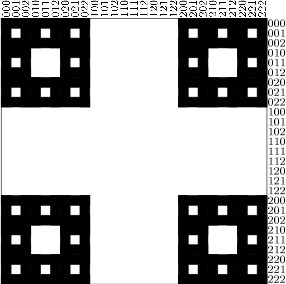
\includegraphics{bildoj/menger-schema07.png}\\ \vspace{0.5cm}
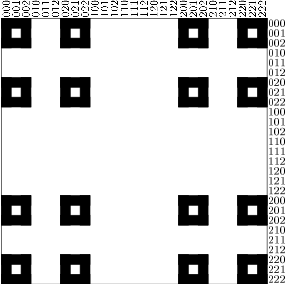
\includegraphics{bildoj/menger-schema08.png}\\ \vspace{0.5cm}
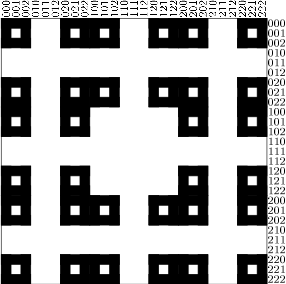
\includegraphics{bildoj/menger-schema09.png}\\ \vspace{0.5cm}
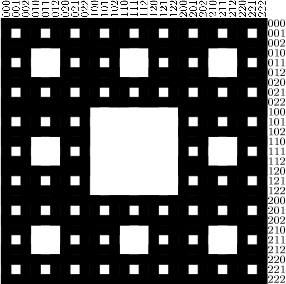
\includegraphics{bildoj/menger-schema10.png}\\ 
\end{center}

Por grafiki spongon je ordo $3$, ni trairos la nombrojn de $1$ ^gis
$27$, tio estas, de $001$ ^gis $222$ je bazo $3$.  Por ^ciu numero,
oni aplikos la ta^ugan sekcion kiun oni portos la^u la $3$ direktoj
$(Ox)$, $(Oy)$ kaj $(Oz)$.

\subsubsection{La kodo}

La jena programo permesas grafiki la solidojn de Menger je ordoj $0$,
$1$, $2$, $3$, $4$.  La nombro de proceduroj estas grava, do mi
klarigos tuj.

\begin{verbatim}
# Grafiki tapiŝon de Sierpinski je ordo :p kaj je amplekso :amplekso
por  tapiŝo :amplekso :p
provizu "unuo :amplekso / (potencon 3 :p)
se :p=0 [ort :amplekso :amplekso haltu]
se :p=1 [ripetu 4 [ort :amplekso :unuo an :amplekso dn 90] haltu]
ripetupor (list "x 1 potencon 3 :p) 
  [lokp "cantorx cantor :x :p []
   # Ne grafiku erojn havantajn unu 1 en la lasta loko
   se  ne (1 = lastan :cantorx)  
     [lokp "nom valorigu senlastan :cantorx "
      grafikuvertikalon :x econ_sendu "map :nom]]  
fino

# Sendu la prezenton je bazo 3 de la nombro x
# p profundeca indekso 3^p
# :list listo malplena ĉe l' komenco

por cantor :x :p :list
se :p=0 [sendu :list] 
lokp "a potencon 3 :p-1
se :x <= :a 
  [sendu cantor :x :p-1 frazon :list 0] 
  [se :x <= 2*:a [sendu cantor :x-:a :p-1 frazon :list 1]
   sendu cantor :x-2*:a :p-1 frazon :list 2]
fino

# Grafiku la numeron x laŭ la konstruskemo difinita en la listo
por grafikuvertikalon :x :list
  l  dn 90  an (:x-1)*:unuo mdn 90 ml des :list
  l mdn 90  an (:x-1)*:unuo  dn 90 an :x*:unuo dn 90 ml des :list
  l mdn 90 man :x*:unuo ml
fino

# Grafiku ortangulon laŭ donitaj dimensiojn
# La plurlatero estas registrita de la 3d-vidigilo
por ort :lo :la
  provizu "nombrilo :nombrilo+1
  por_edro
    ripetu 2 [an :lo dn 90 an :la dn 90]
  fino_edro
fino

# Komencu la malsamajn vertikalojn eblajn por la tapiŝojn je ordo 1 ĝis 4
por pretmap
econ_sendu "map 111 [3 3 3 9 3 3 3 27 3 3 3 9 3 3 3]
econ_sendu "map 110 [9 9 9 27 9 9 9]
econ_sendu "map 101 [3 3 6 3 6 3 3 27 3 3 6 3 6 3 3]
econ_sendu "map 011 [3 3 3 9 3 3 6 3 3 9 3 3 6 3 3 9 3 3 3]
econ_sendu "map 000 [81]
econ_sendu "map 100 [27 27 27]
econ_sendu "map 010 [9 9 18 9 18 9 9]
econ_sendu "map 001 [3 3 6 3 6 3 6 3 6 3 6 3 6 3 6 3 6 3 3]
econ_sendu "map  01 [3 3 6 3 6 3 3]
econ_sendu "map  00 [27]
econ_sendu "map  10 [9 9 9]
econ_sendu "map  11 [3 3 3 9 3 3 3]
econ_sendu "map   1 [3 3 3]
econ_sendu "map   0 [9]
fino

# Se la prezento estas [1 0 1] --> sendu 101
# Se la prezento estas [1 0 2] --> sendu 100
# La eroj de la listo estas kunmetataj en vorton.
# Krome, la 2 estas anstataŭataj de nuloj
por valorigu :list :vort
  se malplena? :list [sendu :vort]
    [lokp "unua unuan :list
     se :unua=2 [lokp "unua 0] 
     lokp "vort vort :vort :unua
     sendu valorigu senunuan :list :vort]
fino

# Desegnu la ortangulojn de ĉiu vertikalo alterne
por des :list
lokp "sumo 0
ripetupor (liston "i 1 kmpt :list) 
   [lokp "ero eron :i :list
    lokp "sumo :ero+:sumo 
    se para? :i [l an :ero*:unuo ml] [ort :ort*:unuo :unuo an :ero*:unuo]]
l man :sumo * :unuo ml
fino

# Testu ĉu nombro estas para
por para? :i
  sendu 0 = resto :i 2
fino

por siertapiŝo :p
  ev perspektive tdk pretmap
  provizu "nombrilo 0
  tapiŝo 810 :p
  tajpu "Nombro\ de\ plurlateroj:\  s :nombrilo 
  tridimensie_vidigu
fino

# Forigas la lastan 1 en la listo :list
por forigulastanunu :list
  ripetupor (list "i kmpt :list 1 minusigan 1) 
    [lokp "ero eron :i :list 
     se :ero=1 [lokp "list anstataŭigu :list :i 0 haltu] [se :ero=2 [haltu]]]
  sendu :list
fino

# Spongo de Menger je amplekso donita kaj je profundeco :p

por menger :amplekso :p
provizu "unuo :amplekso / (potencon 3 :p)
ripetupor (list "z 1 potencon 3 :p) 
  [lokp "cantorz cantor :z :p []
   lokp "last lastan :cantorz
   lokp "cantorz senlantan :cantorz
   se :last=0 [lokp "ordo valorigu forigulastanunu :cantorz "] [lokp "ordo valorigu :cantorz "]
   lokp "ordo vort "tranĉi :ordo
   graf3tapiŝon :amplekso :ordo :z
   l supren 90 an :unuo malsupren 90 ml]
graf3tapiŝon :amplekso :ordo (potencon 3 :p) + 1
fino

# Grafiku la tapiŝojn de Sierpinski je ordo :p
# laŭ ĉiu akso (Ox), (Oy) et (Oz)
# je la alto :z
pour draw3carpet :size :order :z
  l originen
  supren 90 an (:z-1)*:unuo malsupren 90 ml
  skolp bluan ekzek :ordo :amplekso
  l originen
  mdfn 90 an (:z-1)*:unuo malsupren 90 ml
  skolp flavan ekzek :ordo :amplekso
  l originen  
  supren 90 an :amplekso dn 90 an (:z-1)*:unuo malsupren 90 ml
  skolp violruĝan ekzek :ordo :amplekso
fino

# Ĉefa proceduro
# Grafiku spongon de Menger je profundeco :p
por spongo :p
  ev perspektive tdk
  lokp "tempo tempon
  pretmap
  provizu "nombrilo 0
  se :p=0 [kubo 405] [menger 405 :p]
  # Skribu la tempon kaj la nombron de plurlateroj necesaj por konstrui
  tajpu "Nombro\ de\ plurlateroj:\  s :nombrilo
  tajpu "Tempo\ uzita:\  s tempon - :tempo
  tridimensie_vidigu
fino

# Sekcio por la Menger je ordo 2

por tranĉi1 :amplekso
  ripetu 4 [tapiŝu :amplekso/3 1 l an :amplekso dn 90 ml]
fino

por tranĉi0 :amplekso
  tapiŝo :amplekso 2
fino

# Sekcio por la Menger je ordo 3

por tranĉi10 :amplekso
  ripetu 4 [tapiŝo :amplekso/3 2 l an :amplekso dn 90 ml]
fino

por tranĉi01 :amplekso
  ripetu 4 [ripetu 2 [tranĉi1 :amplekso/3 l an :amplekso/3 ml] an :amplekso/3 dn 90]
fino

por tranĉi11 :amplekso
  ripetu 4 [tranĉi1 :amplekso/3 l an :amplekso dn 90 ml]
fino

por tranĉi00 :amplekso
  tapiŝo :amplekso 3
fino

# Sekcio por la Menger je ordo 4

por tranĉi000 :amplekso
  tapiŝo :amplekso 4
fino

por tranĉi100 :amplekso
  ripetu 4 [tapiŝo :amplekso/3 3 l an :amplekso dn 90 ml]
fino

por tranĉi010 :amplekso
  ripetu 4 [ripetu 2 [tranĉi10 :amplekso/3 l an :amplekso/3 ml] an :amplekso/3 dn 90]
fino

por tranĉi001 :amplekso
  ripetu 4 [ripetu 2 [tranĉi01 :amplekso/3 l an :amplekso/3 ml] an :amplekso/3 dn 90]
fino

por tranĉi110 :amplekso
  ripetu 4 [tranĉi10 :amplekso/3 l an :amplekso ml dn 90]
fino

por tranĉi111 :amplekso
  ripetu 4 [tranĉi11 :amplekso/3 l an :amplekso dn 90 ml]
fino

por tranĉi101 :amplekso
  ripetu 4 [tranĉi01 :amplekso/3 l an :amplekso dn 90 ml]
fino

por tranĉi011 :amplekso
  ripetu 4 [ripetu 2 [tranĉi11 :amplekso/3 l an :amplekso/3 ml] an :amplekso/3 dn 90]
fino

por tranĉi :amplekso
  tapiŝo :amplekso 1
fino

por kubo :amplekso
  ripetu 2 
    [skolp bluan  ort :amplekso :amplekso l an :amplekso malsupren 90 ml
     skolp flavan ort :amplekso :amplekso l an :amplekso malsupren 90 ml]
  skolp violruĝan
  l mdfn 90 mdn 90 an :amplekso dn 90 ml ort :amplekso :amplekso
  l dn 90 an :amplekso mdn 90 dfn 90 dn 90 an :amplekso mdn 90 dfn 90 ml ort :amplekso :amplekso
  mdfn 90 mdn 90 an :amplekso dn 90
fino

por kuboj
  ev perspektive tdk
  lokp "tempo tempon
  pretmap
  provizu "nombrilo 0
  ripetu 4 [se komputu = 1 [kubo 405] [menger 405 komputu-1] l an 1000 dn 90 ml]
  # Montru la tempon uzitan kaj la nombron de plurlateroj necesaj por konstrui
  tajpu "Nombro\ de\ plurlateroj:\  s :nombrilo
  tajpu "Tempo\ uzita:\  s tempon - :tempo
  tridimensie_vidigu
fino
\end{verbatim}

Nun, establu la memoron rezervitan por \xlogo\ je 640 MiB: \texttt{spongo 4}
\begin{center}
 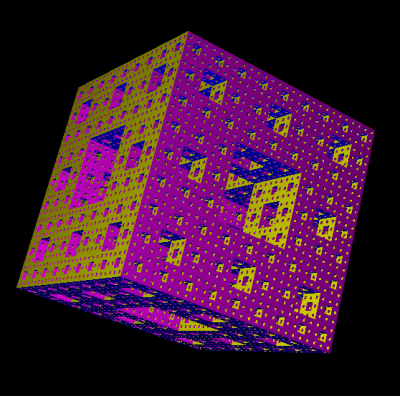
\includegraphics{bildoj/menger-menger4.png}
\end{center}
